\chapter{Metodología}
\label{chap:metodologia}

 %De acuerdo a \cite{Barrett2009}, el modelo WCM...\\

\section{Diseño}
En el IDE EClipse
Funciones enteramente documentadas (Doxigen).
Control de Versiones (GitHub) - graficos de los tiempos de desarrollo. ¿?
En esta tesis se dise\~nar\'a el procedimiento y el prototipo de software para el an\'alisis de una situaci\'on de encuentro entre una misi\'on primaria y un desecho espacial.\\
Partimos de la recepci\'on de un mensaje de alerta, proveniente de un organismo externo (JSpOC), en formato CDM. La primera instancia consiste en extraer la informaci\'on que permita identificar la nave propia, el desecho espacial involucrado y el instante en que se estima el encuentro \ac{TCA}. Ya con esta informaci\'on se puede hacer la solicitud de los TLE a space-track para empezar el an\'alisis de la situaci\'on y se solicitan a Din\'amica Orbital las efem\'erides precisas necesarias.\\
El siguiente paso implica desarrollar un m\'etodo que ajuste los TLE, mejore la estimaci\'on de la posici\'on del desecho y calcule los errores asociados.\\
Finalmente se calcular\'a el par\'ametro de \ac{PoC}, como indicador cuantitativo del nivel del riesgo.\\

Para el desarrollo del prototipo de software ARxCODE, se propone una metodolog\'ia evolutiva incremental, basada en la construcci\'on de distintos m\'odulos que resuelvan las etapas planteadas. Los mismos ir\'an valid\'andose y perfeccion\'andose durante el proceso, de manera independiente pero enmarcados en una arquitectura y dise\~no que se resolver\'a en las primeras etapas.\\
Se listan a continuaci\'on los tres principales m\'odulos a desarrollar:\\ 
%Se plasma una estructura/arquitectura de alto nivel consolidada, cuyas interfaces con: SW de Dinámica Orbital de CUSS y otros entes, queda estipulada y se atomizan estructuras internas, capaces de ser actualizadas y cuyas interacciones sean versátiles.\\

\begin{itemize}
\item M\'odulo de ajuste y correcci\'on de la posici\'on del desecho espacial.\\
\item M\'odulo de c\'alculo de la PoC.\\
\item M\'odulo de administraci\'on del CDM.\\
\item M\'odulo de administraci\'on de los datos provistos por el departamento de Din\'amica Orbital.\\
\end{itemize}
\begin{figure}[!h]
\centering
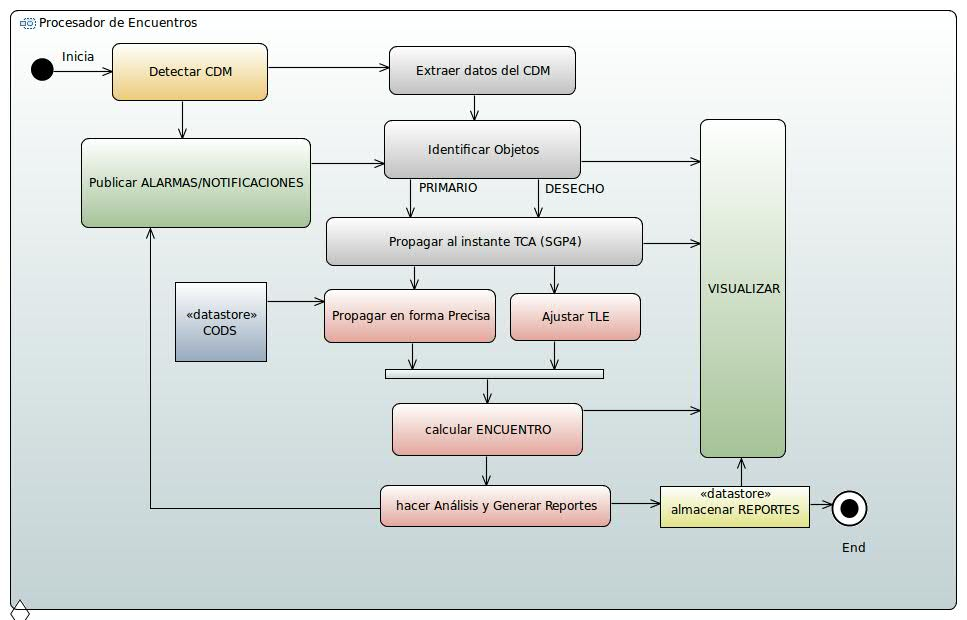
\includegraphics[width=\textwidth]{imagenes/arxcodencuentros}
\caption{Arquitectura de alto nivel del ARxCODE}
\end{figure}


\subsection*{M\'odulo de ajuste y correcci\'on de la posici\'on del desecho.}
Si bien la base de datos de NORAD, pone a disposici\'on p\'ublica la informaci\'on orbital de los objetos en formato TLE, se desconocen los errores asociados a esa determinaci\'on orbital, al igual que los que introduce la propagaci\'on de los mismos con el modelo de propagaci\'on compatible SGP4.\\
En este m\'odulo esta tesis ofrece una nueva variante para la estimaci\'on de errores en la propagaci\'on de \'orbitas de desechos a partir de TLE.\\
Se utiliza el conjunto de los \'ultimos TLE publicados y se calculan las diferencias en la posici\'on, utilizando el \'ultimo TLE m\'as cercano a la fecha del TCA, como se propone en el trabajo de Osweiler \cite{osweiler}. El m\'etodo utiliza un conjunto de TLE de un dado objeto, por el periodo de 2 semanas. A partir de la propagaci\'on con SGP4 calcula las diferencias en las posiciones y velocidades contra un vector de estado estimado, a fin de caracterizar el comportamiento de la varianza y la matriz de covarianza para el TLE m\'as reciente.\\
A partir de esos resultados se realiza un ajuste por m\'inimos cuadrados y se propone una funci\'on de corrección.\\

\subsection*{M\'odulo de cálculo de la PoC.}
%Pasos comunes a todos los m\'etodos.\\
La PoC es el par\'ametro estad\'istico final que nos permitir\'a evaluar cuantitativamente la situaci\'on.\\
Optamos por la PoC ya que muestra mayor confiabilidad que otros par\'ametros, como por ejemplo la miss distance (m\'inima distancia), dado que la miss distance no contempla errores de propagaci\'on y genera sobrestimaci\'on de encuentros.\\
Los c\'alculos probabil\'isticos para este tipo de problemas en tres dimensiones resultan de pesada carga computacional, por lo que conviene usar t\'ecnicas de reducci\'on del problema a dos dimensiones o a un plano de encuentro \cite{foster}. Para el c\'alculo de la PoC se utilizar\'a el m\'etodo de Akella \cite{akellaAlfriend} ya que es conceptualmente simple y aunque tiene un alto costo computacional, es realizable por las m\'aquinas actuales en tiempos menores a un segundo.\\
%El procedimiento general frente a un posible enuentro consiste en propagar las \'orbitas y recalcular la situaci\'on de acercamiento a medida que se aproxima la fecha de la posible colisi\'on. Todo esto  con una antelaci\'on prudencial que permita la planificaci\'on de la maniobra, si \'esta resultara inevitablemente necesaria.

\subsection*{M\'odulo de administraci\'on de los datos provistos por el departamento de Din\'anica Orbital.}
Consiste en la solicitud/extracci\'on de los datos orbitales con la mayor precisi\'on posible que puedan obtenerse, propagados al momento del encuentro.\\
S\'olo ser\'a un m\'odulo de gesti\'on de datos que interactuar\'a con la base de datos de Din\'amica Orbital.\\ 


\subsection*{M\'odulo de administraci\'on del CDM.}
Este m\'odulo ser\'a el encargado de la detecci\'on y el desglose de la informaci\'on del CDM que provee JSpOC.\\
El mismo ofrecer\'a al operador usuario una visualizaci\'on resumida de la situaci\'on con la informaci\'on m\'as importante, y operar\'a de interfaz con el resto del sistema ARxCODE, provey\'endole los datos iniciales necesarios a los siguientes m\'odulos. A saber:\\

\begin{itemize}
\item Identificador de la  misi\'on primaria.
\item Identificador del desecho espacial.
\item TCA.
\item PoC.
\end{itemize}  

Una vez finalizados y validados los m\'odulos, resta la integraci\'on y la verificaci\'on de las distintas interfaces.\\

\section{Entorno de Desarrollo}
...

\section{Desarrollo}
 ...
  \subsection{Interfaz Gr\'afica}


